\chapter{Implémentation et Résultats}
\vspace{3cm}
\minitoc
\clearpage

\label{Chapitre4}

\section{Introduction}
\begin{onehalfspace}
\lettrine[nindent=1em,lines=3]{C}e chapitre est consacré à la réalisation et la concrétisation de nos approches proposées, qui consistent à minimiser l’énergie consommée  dans les  Cloud Computing. Il  aborde l’implémentation de notre stratégie. Nous allons commencer tout  d’abord par fixer l’environnement dans lequel nous avons réalisé notre simulateur. Nous allons définir par la suite  les métriques que nous avons utilisées. Enfin nous allons discuter  et analyser les résultats de la minimisation des migrations des machines virtuelles dans le Cloud Computing que nous avons obtenus.

\end{onehalfspace}
\section{Langage et environnement de développement}
\begin{onehalfspace}
L'environnement de développement est un facteur important qui doit être détaillé pour connaître dans quelles situations, le même travail peut être reproduit. La stratégie proposée dans le cadre de ce travail a été implémentée et testée dans l'environnement suivant :\medskip

\begin{itemize}
\item \textbf{Caractéristiques matérielles et logicielles du PC utilisé :} Nous avons développé notre application sur une machine avec un processeur Intel(R) Core(TM)i3-3110M CPU, une vitesse de 2.40Ghz et une capacité mémoire de 4GB. Le simulateur est  sous Windows 8.1 de 64bits.
\item \textbf{Simulateur utilisé :} CloudSim.
\item \textbf{Langage utilisé :} Java.
\item \textbf{IDE utilisé :} NetBeans.
\end{itemize}
\end{onehalfspace}
\subsection{Langage de programmation Java}
\begin{onehalfspace}
Java est à la fois un langage de programmation informatique orienté objet et un environnement
d’exécution portable. Il est céé par James Gosling et Patrick Naughton employés
de Sun Microsystems avec le soutien de Bill Joy (co-fondateur de Sun Microsystems en
1982), présenté officiellement le 23 mai 1995 au SunWorld \cite{ref39}.\medskip

Le langage Java a la particularité principale que les logiciels écrits avec ce dernier sont
très facilement portables sur plusieurs systèmes d’exploitation tels que : Unix, Microsoft
Windows, Mac OS ou Linux avec ou sans modifications. C’est la plate-forme qui
garantit la portabilité des applications développées en Java \cite{ref39}.\medskip

Les applications Java peuvent être exécutées sur tous les systèmes d’exploitation pour
lesquels a été développée une plate-forme Java dont le nom technique est JRE (Java Runtime
Environment - Environnement d’exécution Java). Cette dernière est constituée d’une
JVM (Java Virtual Machine - Machine Virtuelle Java), le programme qui interprète le code
Java et le convertit en code natif. Mais le JRE est surtout constitué d’une bibliothèque
standard à partir de laquelle doivent être développés tous les programmes en Java. C’est
la garantie de portabilité qui a fait la réussite de Java dans les architectures client-serveur
en facilitant la migration entre serveurs, ce qui est très difficile pour les gros systèmes \cite{ref40}.\medskip

Java est devenu aujourd’hui une direction incontournable dans le monde de la programmation
parmi les différentes caractéristiques qui sont attribuées à son succès , nous avons \cite{ref39} :\medskip

\begin{itemize}
\item L’indépendance de toute plate-forme : le code reste indépendant de la machine sur
laquelle il s’exécute. Il est possible d’exécuter des programmes Java sur tous les
environnements qui possèdent une Java Virtual Machine.
\item Java est également portable, permettant à la simulation d’être distribuée facilement
sans avoir à recompiler le code pour les différents systèmes.
\item Le code est structuré dans plusieurs classes dont chacune traite une partie différente
de la simulation.
\item Il assure la gestion dynamique de la mémoire.
\item Java est multitâches : il permet l’utilisation de Threads qui sont des unités d’exécution
isolées.

\end{itemize}

Aussi, une des principales raisons de ce choix est que le simulateur CloudSim est développé
avec ce langage.

\end{onehalfspace}

\subsection{Environnements de développement}
\begin{onehalfspace}
NetBeans est un environnement de développement intégré (EDI), placé en Open Source par Sun en Juin 2000. En plus de Java, NetBeans permet également de supporter différents autres langages, comme Python, C, C + +, JavaScript, XML, Ruby, PHP et HTML téléchargeable du site : \url{https ://netbeans.org/downloads}. Il comprend toutes les caractéristiques d’un IDE moderne (éditeur en couleur, projets multi-langage, refactoring, éditeur graphique d’interfaces et de pages Web).\medskip

Conçu en Java, NetBeans est disponible sous Windows, Linux, Solaris, MacOSX ou sous une version indépendante des systèmes d’exploitation (requérant une machine virtuelle Java).\medskip

De plus, NetBeans est écrit en Open Source, téléchargeable directement du site \url{http ://java.sun.com}. Il est puissant et compatible avec toutes les nouvelles technologies Java (les technologies Java EE, les bases de données, UML, XML, ...).
\end{onehalfspace}

\subsection{Simulateur CloudSim}
\begin{onehalfspace}
CloudSim est une nouvelle structure de simulation généralisée et extensible qui permet
la modélisation des environnements hétérogènes, la simulation et l’expérimentation de
Cloud émergent des infrastructures de calcul et des services d’application. Il offre les
fonctionnalités suivantes :\medskip
\begin{itemize}
\item Une plate-forme indépendante pour la modélisation des Data Centers, des Brokers, de l'ordonnancement et des politiques d'allocation des ressources;
\item Support pour la modélisation et la simulation à grande échelle d’infrastructure de
Cloud Computing, y compris des centres de données sur un seul noeud physiques.
\end{itemize}\medskip

Parmi les principales caractéristiques de CloudSim, nous pouvons citer :
\begin{itemize}
\item La flexibilité pour commuter entre l’allocation en espace et en temps
partagé 
et la prise en charge de la répartition des coeurs de traitement aux services
virtualisés;
\item La disponibilité d’un moteur de virtualisation qui facilite la création et la gestion
indépendante des services ainsi que l’hébergement des services virtualisés sur un
noeud d’un Datacenter ;
\item Un support pour la simulation des connexions réseau entre les éléments du système
de simulation ;
\item Simulation de la définition de matériel de centre de traitement des données (Datacenter)
en termes de machines physiques composées de processeurs, de dispositifs
de stockage, de mémoire et de largeur de bande interne ;
\item Simulation des spécifications, de la création et de la destruction de machines virtuelles
;
\item Simulation de l’exécution des programmes utilisateurs ou des demandes (Cloudlet)
sur les machines virtuelles.

\end{itemize}
Nous avons utilisé pour la réalisation de notre travail la version du simulateur CloudSim 2.1.1 téléchargeable du site : \url{https ://code.google.com/p/cloudsim/downloads/list}.
\end{onehalfspace}
\subsubsection{Architecture de CloudSim}
\begin{onehalfspace}
La structure logicielle de CloudSim et ses composants sont représentés par une architecture en couches comme c'est montré dans la Figure \ref{Architecture du système}. Les premières versions de CloudSim utilise SimJava, un moteur de simulation d'événement discret qui met en oeuvre les principales fonctionnalités requises pour des structures de simulation de haut niveau. Parmi les fonctionnalités, nous avons la formation d'une file d'attente et le traitement d'événements, la création de composants système (les services, les machines (Host), le centre de données (Datacenter), le courtier (Broker), les machines virtuelles), la communication entre les composants et la gestion de l'horloge de simulation :

\begin{figure}[!h]
\begin{center}
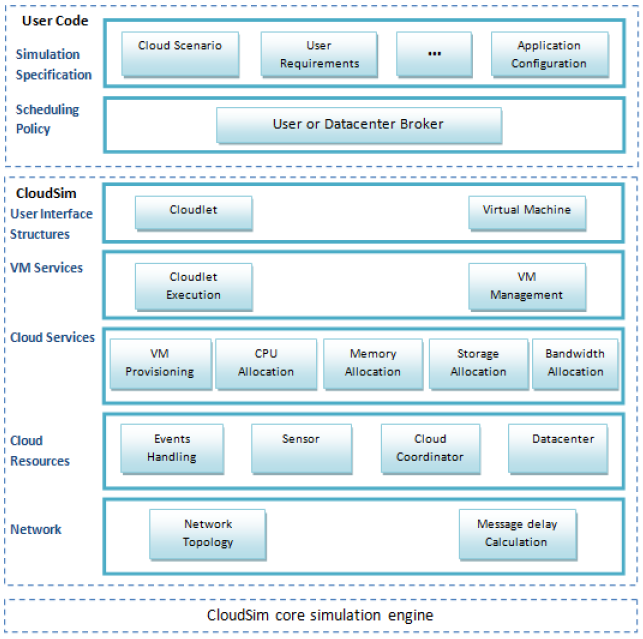
\includegraphics[scale=0.5]{figures/5.png} 
\end{center}
\caption{Architecture de CloudSim \cite{ref41}}
\label{ArchitecturedeCloudSim}
\end{figure}

\end{onehalfspace}

\subsubsection{Classes de CloudSim}

\begin{onehalfspace}
Le simulateur CloudSim est composé de plusieurs classes que nous pouvons classer en deux catégories : des classes qui modélisent les entités comme le Data Center, le Broker, etc. Et des classes modélisant les politiques d'allocation.

Parmi les classes fondamentales qui forment les blocs constitutifs du simulateur CloudSim comme est présenté dans la Figure \ref{ClassCloudSim} , nous pouvons citer seulement celles utilisées :
\begin{figure}[!h]
\begin{center}
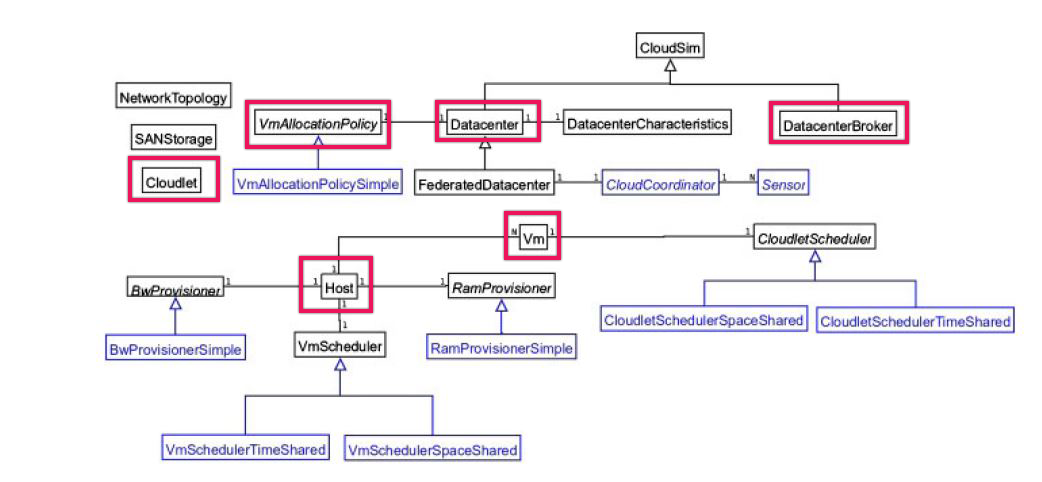
\includegraphics[scale=0.52]{figures/cloudsimclass.png} 
\end{center}
\caption{Diagramme de classe de la conception de simulateur CloudSim}
\label{ClassCloudSim}
\end{figure}
 
\begin{enumerate} [label=\Alph*.      ]
\item \textbf{Cloudlet :} Cette classe modélise les services d'application du Cloud (comme la livraison, réseaux
sociaux, et le workflow d'affaires). CloudSim représente la complexité d'une application en fonction de ses besoins informatiques. Chaque service d'application a une taille d'instruction pré-assigne et la quantité de flux de transfert de données qu'il doit entreprendre au cours de son cycle de vie. Cette classe peut également être étendu pour supporter la modélisation de la performance et d’autres paramètres de composition pour les applications telles que les transactions dans les applications orientées base de données \cite{ref45}.
\item \textbf{Datacenter :} Cette classe modélise les services au niveau des infrastructures de base (matériel) qui sont offerts par les fournisseurs de Cloud (Amazon, Azure, App Engine). Elle encapsule un ensemble de hôtes qui peuvent être soit homogènes ou hétérogènes par rapport à leurs configurations matérielles (mémoire, noyaux, capacité et stockage) \cite{ref45}.
\item \textbf{DatacenterBroker :} Cette classe modélise le Broker, qui est responsable de la médiation entre les utilisateurs et les prestataires de service selon les conditions de QoS des utilisateurs et il déploie les tâches de service à travers les Clouds. Le Boker au nom des utilisateurs, agit sur les prestataires du service approprié du cloud par le service d’information du Cloud CIS (Cloud Information Services) et négocie avec eux pour une allocation des ressources qui répond aux besoins de QoS des utilisateurs. Les chercheurs et développeurs des systèmes doivent étendre cette classe pour évaluer et tester les politiques de courtage personnalisées. \cite{ref45}.
\item \textbf{DatacenterCharacteristics :} Cette classe contient les informations sur la configuration des ressources des centres de données \cite{ref45}. 
\item \textbf{Host :} Cette classe modélise une ressource physique comme le serveur de stockage ou de calcul. Elle encapsule des informations importantes telles que la quantité de mémoire et de stockage, le type de coeurs de traitement (pour représenter une machine multi-core), une politique d’allocation pour le partage de la puissance du traitement entre les machines virtuelles et les politiques d’approvisionnement de mémoire et de bande passante pour les machines virtuelles \cite{ref45}.
\item \textbf{SimEntity :} Il s'agit d'une classe abstraite, elle représente l’entité de simulation qui est capable d'envoyer des messages à d'autres entités et de gérer les messages reçues ainsi que les événements. Toutes les entités doivent étendre cette classe et redéfinir ses trois principales méthodes : \textit{startEntity()}, \textit{processEvent()} et \textit{shutdownEntity()}. Ces méthodes définissent les actions pour l'initialisation de l’entité, le traitement des événements et la destruction de l’entité \cite{ref45}.
\item \textbf{VM :} Cette classe représente une instance de machine virtuelle (VM) qui est gérée et hébergée par une machine physique (hôte). Chaque composant VM a accès à un composant qui stocke les caractéristiques suivantes liées à une VM telles que: mémoire accessible, le processeur, capacité de stockage, et les politiques de provisionnement interne de la machine virtuelle qui est étendu à partir d'un composant abstrait appelé le CloudletScheduler \cite{ref45}.
\item \textbf{VMAllocationPolicy :} C'est une classe abstraite implémentée par un composant hôte qui modélise les politiques (d'espace partagé, de temps partagé) exigées pour allouer la puissance de traitement aux VMs. Les fonctionnalités de cette classe peuvent facilement être ignorées pour accommoder des politiques spécifiques à l'application de partage de processeur \cite{ref45}.
\item \textbf{VMProvisioner :} Cette classe abstraite représente la politique d'approvisionnement qu'un moniteur de VM utilisé pour allouer les VMs aux hôtes. La VMProvisioner sélectionne l’hôte qui répond à la quantité de mémoire demandée, le stockage pour le déploiement de la VM \cite{ref45}.
\end{enumerate} 
\end{onehalfspace}


\section{Description du fonctionnement de notre logiciel}
\begin{onehalfspace}
Nous présentons dans cette partie une vue globale de notre simulateur en détaillant les différentes étapes à effectuer pour réaliser une simulation.

Selon le diagramme de la Figure \ref{DiAFL}, la simulation commence après :

\begin{enumerate}
\item \textbf{Création du Cloud : } étape permettant de créer l’architecture Cloud en spécifiant le nombre de DataCenters.
\item \textbf{Configuration de Data Center : } Cette étape permet de spécifier les caractéristiques du Data Center telle que le nombre de nœuds physiques, la bande passante, etc.
\item  \textbf{Configuration des PMs : } Cette étape permet de créer une machine physique et spécifier ses caractéristique telle que nombre de processeurs, la capacité de stockage, etc.
\item  \textbf{Configuration des VMs : } Cette étape permet de créer une machine virtuelle.
\end{enumerate}
\begin{figure}[!h]
\begin{center}
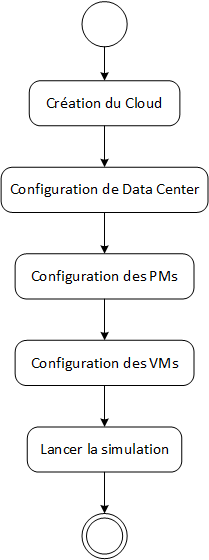
\includegraphics[scale=0.95]{figures/9.png} 
\end{center}
\caption{Diagramme d’activité du fonctionnement de notre logiciel}
\label{DiAFL}
\end{figure}
\end{onehalfspace}
\section{Implémentation}
\begin{onehalfspace}
Dans cette partie, nous allons nous intéresser à la démonstration de notre application à travers un exemple en faisant référence à quelques interfaces graphiques.
\subsection{Accès à l’interface}
La version de CloudSim n’a pas d’interface graphique, son exécution se fait sur la console donc nous avons créé une interface qui facilite l’accès au simulateur. L’interface doit faire appel à CloudSim ainsi qu’aux différentes approches qui se trouvent dans différents packages.\medskip

La Figure \ref{InterfacePrincipale} représente la première interface de notre simulateur qui apparaît à l'utilisateur. 

\begin{figure}[!h]
\begin{center}
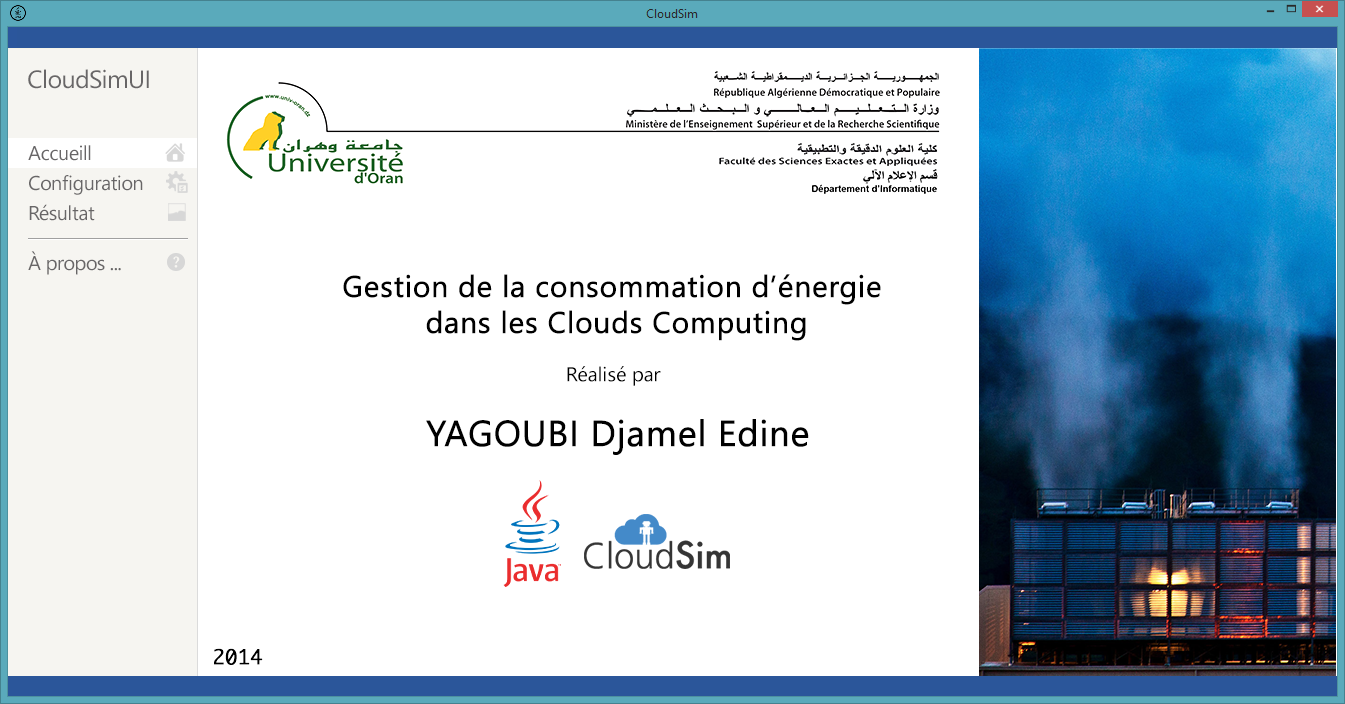
\includegraphics[scale=0.4]{figures/inf1.png} 
\end{center}
\caption{Interface principale}
\label{InterfacePrincipale}
\end{figure}

\subsection{Configuration de Simulation}
La première action à effectuer est la configuration des composants du Cloud. Cette configuration est réalisée en quatre étapes :
\subsubsection{Configuration du Data Center}

Cette étape consiste à faire entrer les caractéristiques du Data Center (voir Figure \ref{ConfigurationdeDatacenter} ) comme : le nom du Data Center, l'architecture de système d'exploitation, le coût de traitement, le coût de la mémoire, le coût de stockage, le coût de la bande passante , l'intervalle de l'ordonnancement et le système d'exploitation. 

\begin{figure}[!h]
\begin{center}
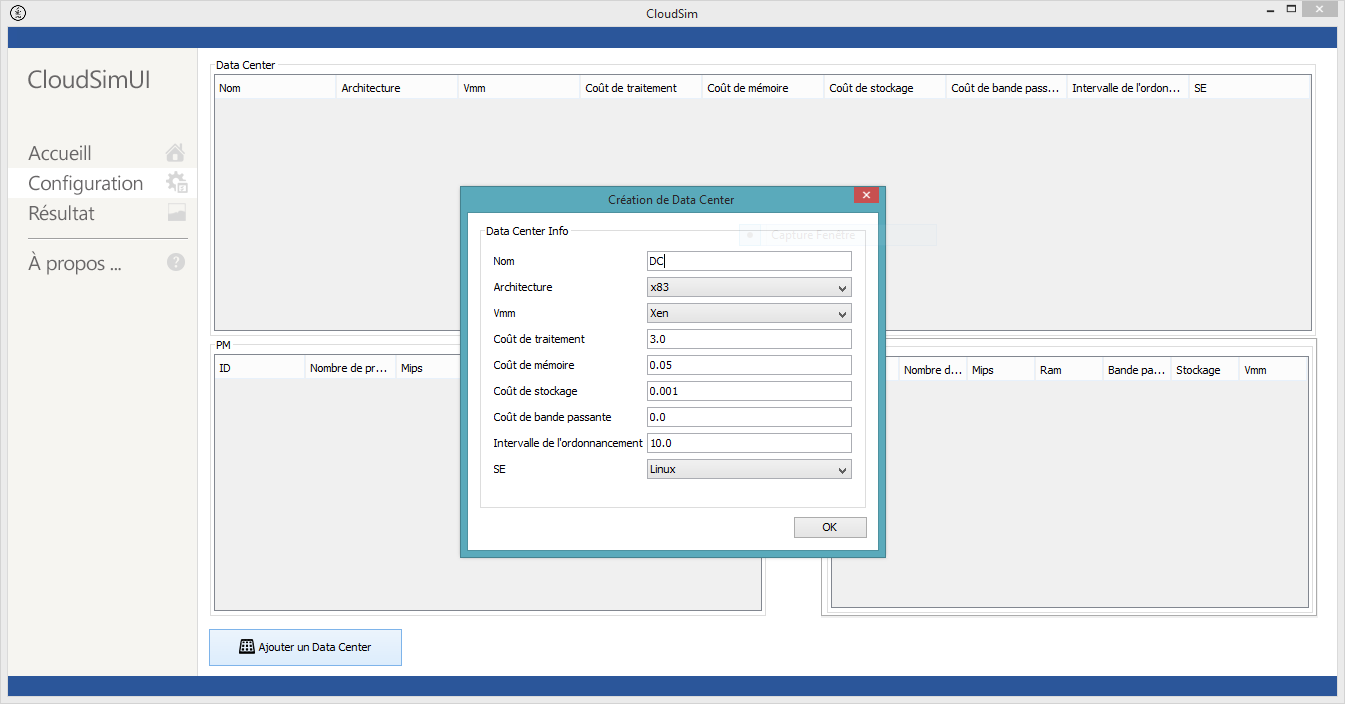
\includegraphics[scale=0.4]{figures/inf2.png} 
\end{center}
\caption{Configuration du Data Center}
\label{ConfigurationdeDatacenter}
\end{figure}
\subsubsection{Configuration des machines physiques}
La Figure \ref{Configurationdesmachinesphysiques} représente l’étape de création des machines physiques. Le bouton \textit{\textbf{Ajouter des machines physiques}} permet de créer des machines physiques hétérogènes en précisant le nombre des hôtes, nombre de processeur, MIPS, RAM, capacité de stockage et la bande passante.
\clearpage
\begin{figure}[!h]
\begin{center}
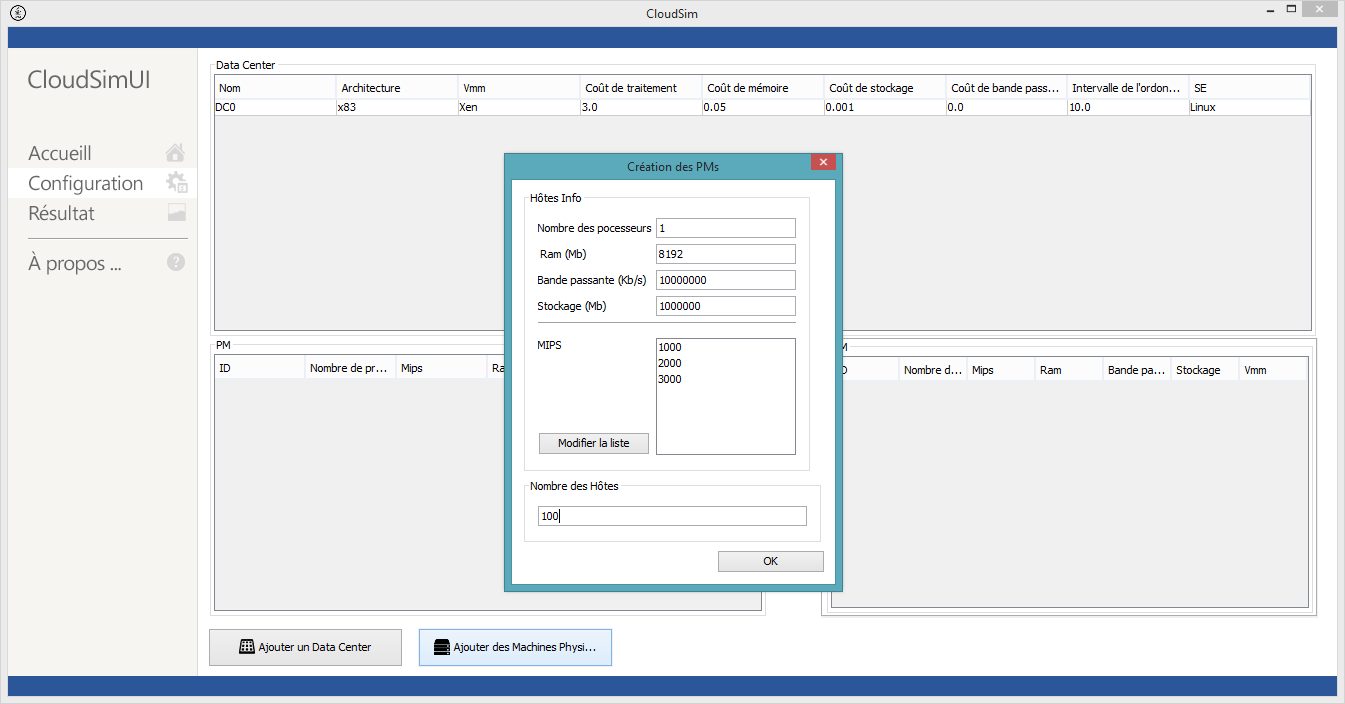
\includegraphics[scale=0.4]{figures/inf3.png} 
\end{center}
\caption{Configuration des machines physiques}
\label{Configurationdesmachinesphysiques}
\end{figure}

\subsubsection{Configuration des machines virtuelles et Cloudlets}

La création des Cloudlets et des machines virtuelles hétérogènes  se fait en cliquant sur le bouton \textbf{Ajouter des machines virtuelles} (voir Figure \ref{CMVCs}). Pour cela, il faut  préciser le nombre des Cloudlets, le nombre de processeur, MIPS, RAM, capacité de stockage, la bande passante, taille de cloudlet, taille de fiché de cloudlet et la  taille de sortie de cloudlet.

\clearpage
\begin{figure}[!h]
\begin{center}
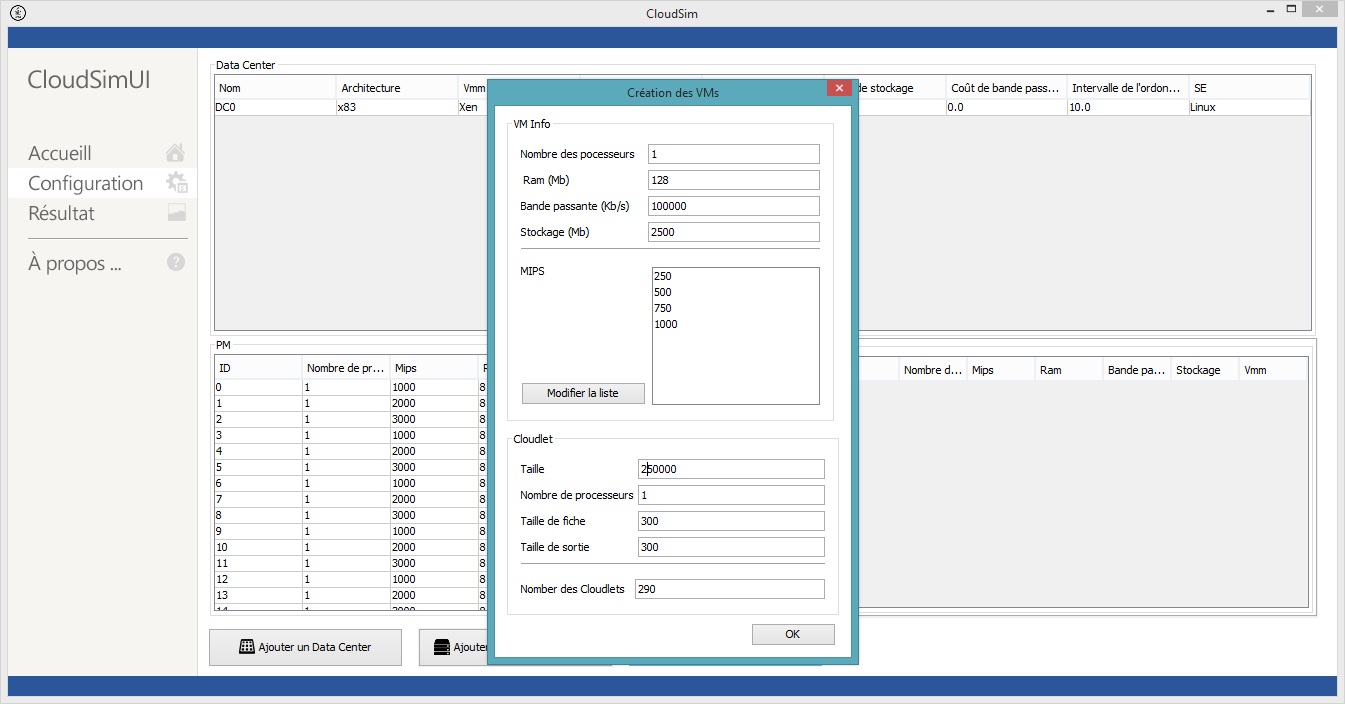
\includegraphics[scale=0.4]{figures/inf4.png} 
\end{center}
\caption{Configuration des machines virtuelles et Cloudlets}
\label{CMVCs}
\end{figure}

\subsubsection{Lancement de la simulation}
Le bouton \textit{\textbf{Lancer la simulation}} illustré dans la Figure \ref{LDS} permet de choisir les paramètres de simulation en spécifiant le nombre de simulations, le seuil de l'approche \textit{ \textbf{Single Threshold }} et les seuils supérieurs et inférieurs de l'approche  \textit{\textbf{Fixed Double Threshold}}. Nous pouvons lancer les simulations en cliquant sur le bouton \textit{\textbf{OK}}. 
\clearpage
\begin{figure}[!h]
\begin{center}
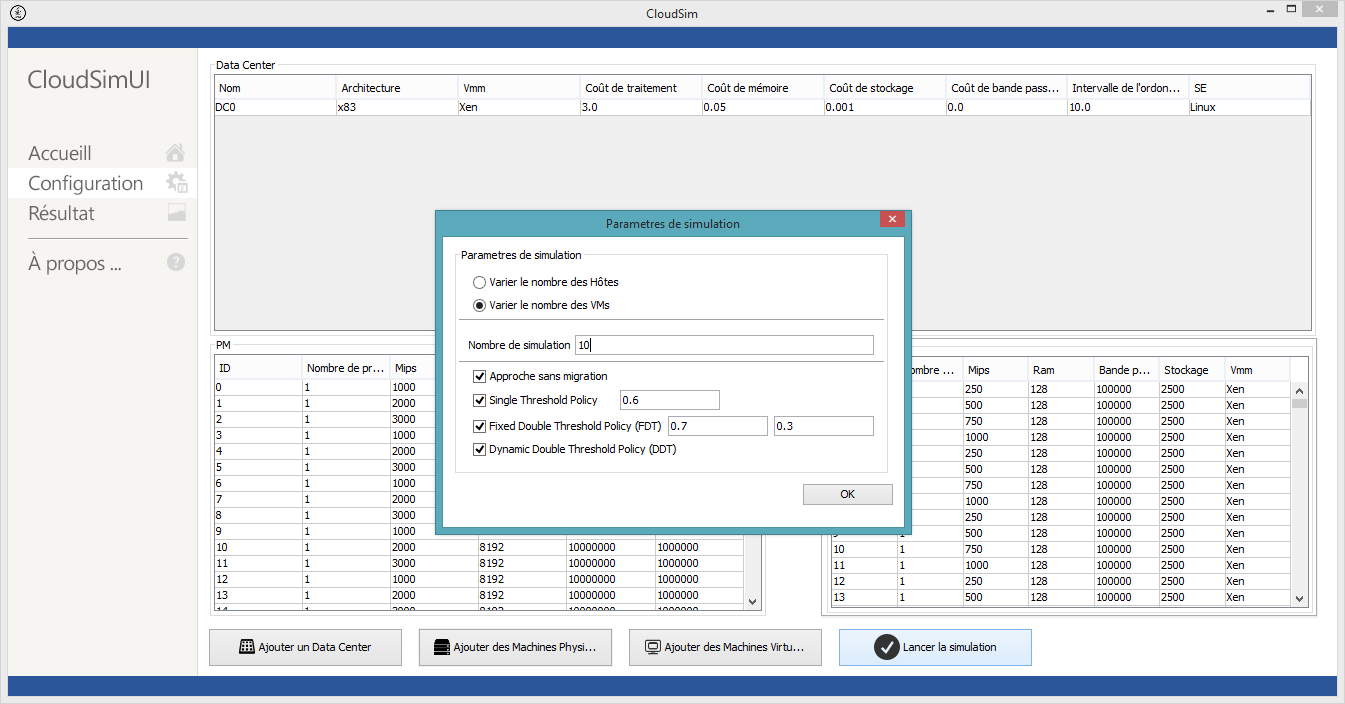
\includegraphics[scale=0.4]{figures/inf5.png} 
\end{center}
\caption{Lancement de la simulation}
\label{LDS}
\end{figure}

\subsubsection{Résultat}
Le bouton « Résultat » permet à son tour d’afficher les résultats des simulations représentées dans le graphe (voir Figure \ref{Résultat}) à l’aide d’un API java JFreeChart\footnote{\textbf{JFreeChart} est une API Java permettant de créer des graphiques et des diagrammes de très bonne qualité.}.
\clearpage
\begin{figure}[!h]
\begin{center}
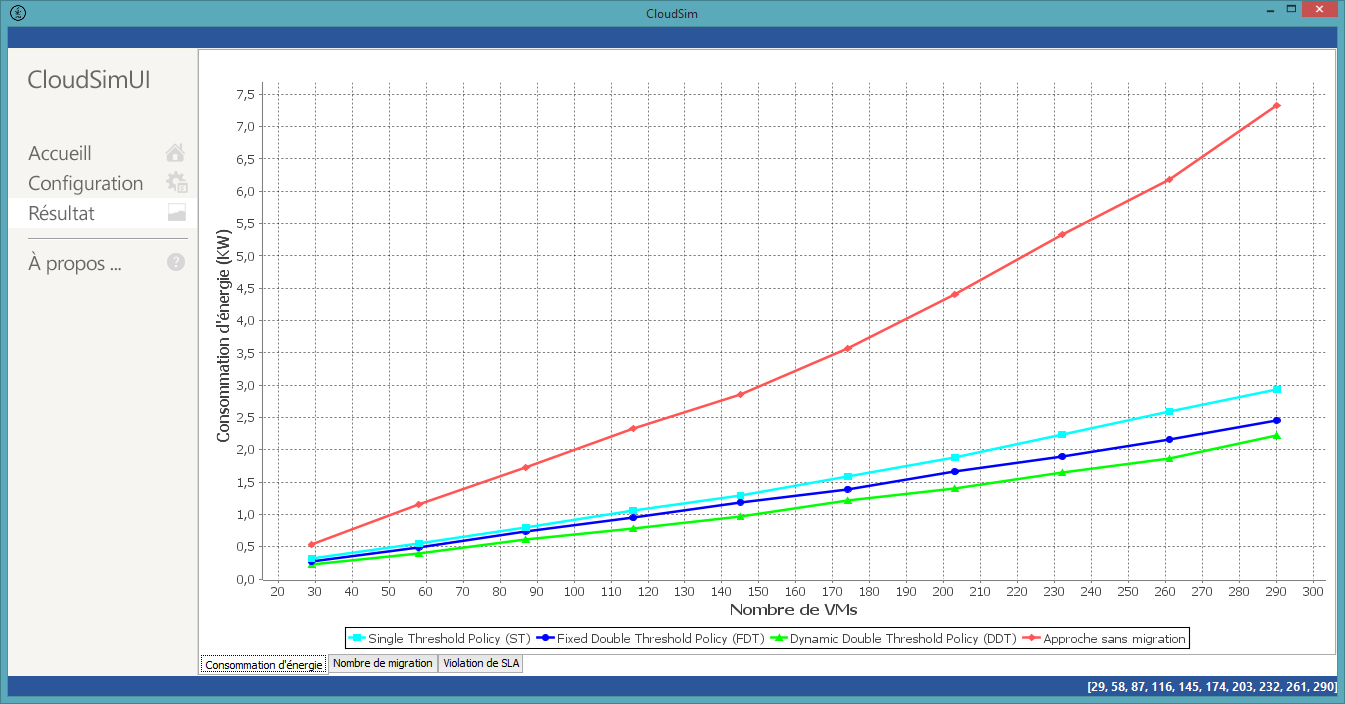
\includegraphics[scale=0.4]{figures/inf6.png} 
\end{center}
\caption{Résultat}
\label{Résultat}
\end{figure}

\end{onehalfspace}

\section{Expérimentations}

\begin{onehalfspace}
Pour mettre en valeur les apports de nos approches, nous allons se focaliser sur les métriques suivantes : l’énergie consommée, nombre de migrations et violations de SLA. Dans le but d’étudier le comportement de nos propositions et d’analyser ses résultats obtenus par la simulation, nous allons les comparer à deux approches: l’approche sans migration et l’approche \textit{\textbf{Single Threshold}}. Plusieurs séries de simulation ont été lancées selon plusieurs paramètres.

\subsection{Expérience 1 : Variation du nombre de VMs}
Dans cette simulation, nous avons créé un Data Center contenant 100 hôtes hétérogène, Chaque hôte posséde 1 processeur avec une vitesse variante en MIPS (1000, 2000 ou 3000), 8GB de mémoire, 1TB de stockage et consomme de 175 W avec 0\% d'utilisation du processeur jusqu'à 250 W avec 100\% d'utilisation du processeur. Le Broker fait varier un nombre de VMs hétérogène de 29 à 290 pour chaque VM a 1 processeur avec une vitesse variante en MIPS (250, 500, 750 ou 1000), 128MB de mémoire, 1GB de stockage. Nous avons considéré le seuil de l’approche \textbf{Single Threshold} comme 0.6 d'après \cite{ref43}. Comme seuil supérieur et inférieur  de l’approche \textbf{Fixed Double Threshold} , nous avons pris les valeurs 0,6 et 0,3 respectivement d'après \cite{ref43}.
\subsubsection{Consommation d’énergie}
Pour analyser la consommation d’énergie, les résultats obtenus par les simulations sont résumés numériquement dans les tableaux \ref{tab2} et \ref{GAIN1} et schématisés par la Figure \ref{InNVMEn}.\\


\begin{center}
{\scriptsize   \begin{tabular}{|p{3.5cm}|c|c|c|c|c|c|c|c|c|c|}
\hline
      \centering     Nombre de VMs &  29& 58& 87& 116& 145& 174& 203& 232& 261& 290\\
\hline
     \centering       Approche sans migration &  5.21& 10.83& 16.61& 22.45& 27.57& 33.69& 38.65& 44.15& 50.22& 60.55\\
\hline
      \centering      Single Threshold &  4.69& 9.30& 13.78& 18.39& 22.80& 27.78& 33.21& 38.14& 43.97& 49.98\\
\hline
      \centering      Fixed Double Threshold &  3.90& 7.86& 11.73& 15.76& 19.53& 23.66& 27.62& 32.06& 36.38& 40.93\\
\hline
      \centering     Dynamic Double Threshold &  3.67& 7.19& 10.56& 13.89& 17.62& 20.63& 24.61& 27.97& 31.91& 36.26\\
\hline
\end{tabular}}
\captionof{table}{Comparaison entre la consommation d’énergie des quatre approches}
\label{tab2}
\end{center}


Le tableau \ref{GAIN1} montre la différence entre les quatre approches, où nous pouvons déduire que notre approche \textbf{Dynamic Double Threshold} a réduit l’énergie avec un gain moyen de 36,21\% par rapport à l'approche sans migration, un gain moyen de 24,81\% par rapport à l'approche \textbf{Single Threshold} et un gain moyen de 10,61\% par rapport à l'approche \textbf{Fixed Double Threshold}.\\


\begin{center}
{\scriptsize   \begin{tabular}{|p{3.5cm}|c|}
\hline
      \centering      Nom de l’approche &  Gain\\
\hline
     \centering       Approche sans migration et Dynamic Double Threshold &  36,21\%\\
\hline
      \centering      Single Threshold et Dynamic Double Threshold&  24,81\%\\
\hline
      \centering      Fixed Double Threshold et Dynamic Double Threshold&  10,61\%\\
\hline
\end{tabular}}
\captionof{table}{Comparaison entre la consommation d’énergie des quatre approches}
\label{GAIN1}
\end{center}



Nous remarquons dans cette simulation représentée par la Figure \ref{InNVMEn}, une augmentation d’énergie consommée par rapport aux quatre approches. Nous pouvons dire que cela est dû à l’augmentation du nombre de VMs. Nous remarquons aussi que les courbes des approches proposées (la courbe bleue et la courbe verte) se trouvent au-dessous des courbes des autres approches (la courbe rouge et la courbe cyan). Donc nos propositions sont bien meilleure par rapport aux autres approches et elle permettent d’économiser de l’énergie. Nous déduisons que notre approche dégage moins de chaleur, cela permet de la  classer  parmi les approches de l'informatique verte. 

\begin{figure}[!h]
\begin{center}
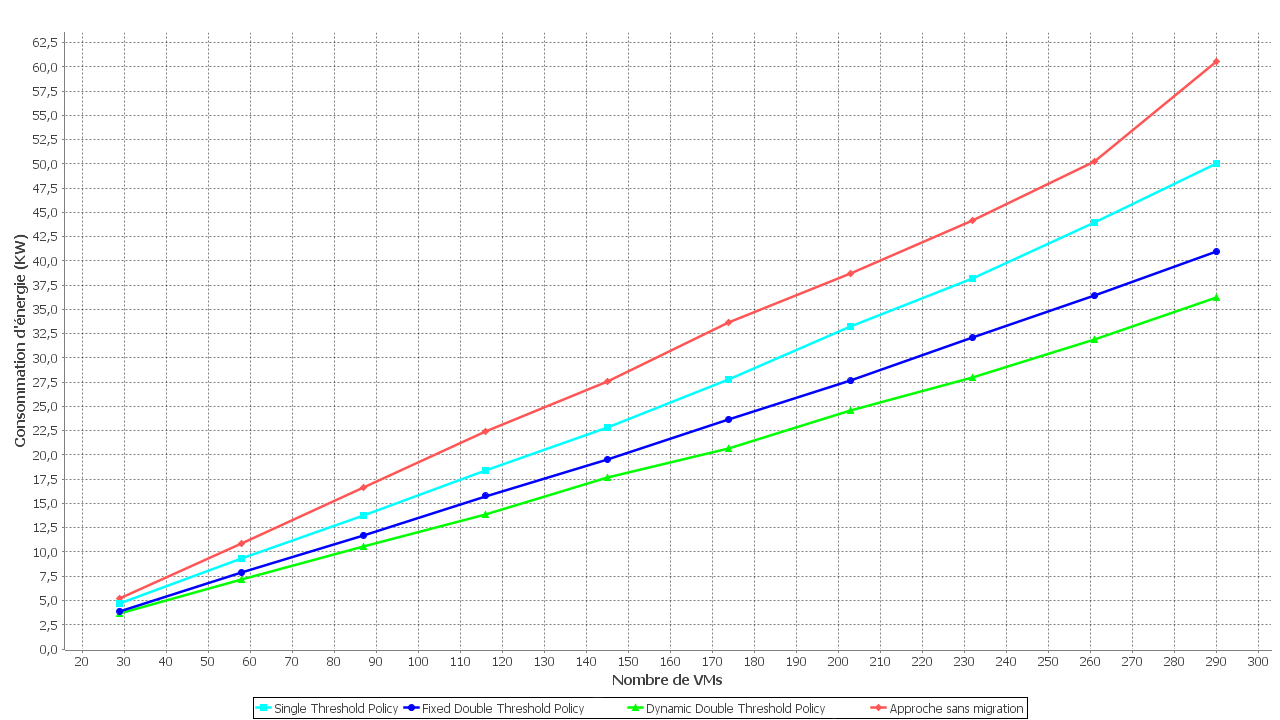
\includegraphics[scale=0.35]{figures/sh1.png} 
\end{center}
\caption{Influence du nombre des VMs sur l’énergie}
\label{InNVMEn}
\end{figure}


\subsubsection{Nombre de migrations}
Dans cette série de simulations représentée par la Figure \ref{InNVMEnM}, nous remarquons  une augmentation du nombre de migrations dans les  trois approches. Nous pouvons justifier cela par l’augmentation du nombre des VMs.
Nous remarquons aussi qu’avec l’augmentation du nombre de VMs, la différence entre les courbes augmente et les courbes des approches proposées se trouvent au-dessous de la courbe de l’approche \textbf{Single Threshold}. Donc les approches \textbf{Fixed Double Threshold} et \textbf{Dynamic Double Threshold} sont bien meilleures que l’approche Single Threshold et permettent de minimiser le nombre de migrations.

Le tableau \ref{tab3} compare entre les trois approches (\textbf{Single Threshold}, \textbf{Fixed Double Threshold} et \textbf{ Dynamic Double Threshold}). Nous remarquons  que les  approches proposées réduisent le nombre de migration des VMs par rapport à l’approche \textbf{single Threshold}.

\begin{center}
{\scriptsize   \begin{tabular}{|p{2.5cm}|c|c|c|c|c|c|c|c|c|c|}
\hline
      \centering     Nombre de VMs &  29& 58& 87& 116& 145& 174& 203& 232& 261& 290\\
\hline
      \centering      Single Threshold &  4589& 10885& 16807& 22970& 29323& 35502& 41896& 48240& 54692& 61072\\
\hline
      \centering      Fixed Double Threshold &  2060& 5638& 10049& 15038& 18630& 25452& 29861& 34003& 40886& 44736\\
\hline
      \centering     Dynamic Double Threshold &  415& 1446& 1976& 2674& 3715& 4363& 5291& 6714& 7448& 9346\\
\hline
\end{tabular}}
\captionof{table}{Comparaison entre le nombre de migrations des trois approches}
\label{tab3}
\end{center}

\begin{figure}[!h]
\begin{center}
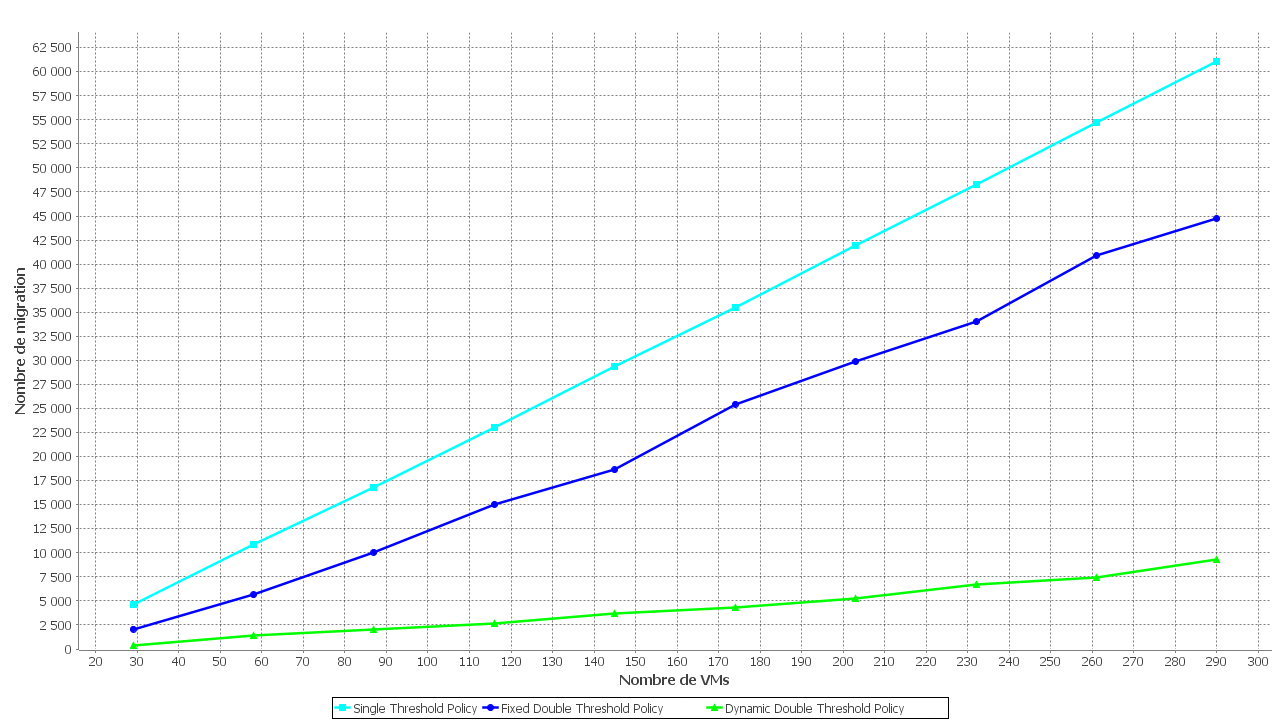
\includegraphics[scale=0.35]{figures/sh2.png} 
\end{center}
\caption{Influence du nombre des VMs sur le nombre de migrations}
\label{InNVMEnM}
\end{figure}

Le tableau \ref{GAIN2} montre la différence entre les trois approches, où nous pouvons déduire que notre approche \textbf{Dynamic Double Threshold} a réduit le nombre de migrations avec un gain moyen de 87,38\% par rapport à l'approche \textbf{Single Threshold} et un gain moyen de 80,31\% par rapport à l'approche \textbf{Fixed Double Threshold}.\\


\begin{center}
{\scriptsize   \begin{tabular}{|p{3.5cm}|c|}
\hline
      \centering      Nom de l’approche &  Gain\\
\hline
      \centering      Single Threshold et Dynamic Double Threshold&  87,38\%\\
\hline
      \centering      Fixed Double Threshold et Dynamic Double Threshold&  80,31\%\\
\hline
\end{tabular}}
\captionof{table}{Comparaison entre le nombre de migrations des trois approches}
\label{GAIN2}
\end{center}

\subsubsection{Violation de SLA}
La Figure \ref{InNVMEV} résultante du tableau \ref{tab4} montre le comportement des deux approches par rapport au nombre de violations de SLA. Nous remarquons que les courbes des approches \textbf{Fixed Double Threshold} et \textbf{Dynamic Double Threshold} se trouvent au-dessous de la courbe de l’approche \textbf{Single Threshold}. Nous remarquons aussi qu’avec l’augmentation du nombre de VMs, la différence entre les courbes augmente. Donc les approches \textbf{Fixed Double Threshold} et \textbf{Dynamic Double Threshold} permettent de minimiser le nombre de violations de SLA.

\begin{center}
{\scriptsize   \begin{tabular}{|p{2.5cm}|c|c|c|c|c|c|c|c|c|c|}
\hline
      \centering     Nombre de VMs &  29& 58& 87& 116& 145& 174& 203& 232& 261& 290\\
\hline
      \centering      Single Threshold &  4786& 12420& 20010& 27810& 36461& 44241& 52839& 61543& 70830& 79590\\
\hline
      \centering      Fixed Double Threshold &  3023& 8827& 16125& 23449& 30604& 40439& 48878& 55547& 67278& 75000\\
\hline
      \centering     Dynamic Double Threshold &  993& 3840& 6402& 8112& 12821& 15182& 17325& 22882& 26316& 29488\\
\hline
\end{tabular}}
\captionof{table}{Comparaison entre le nombre de violations de SLA des trois approches}
\label{tab4}
\end{center}
\clearpage
\begin{figure}[!h]
\begin{center}
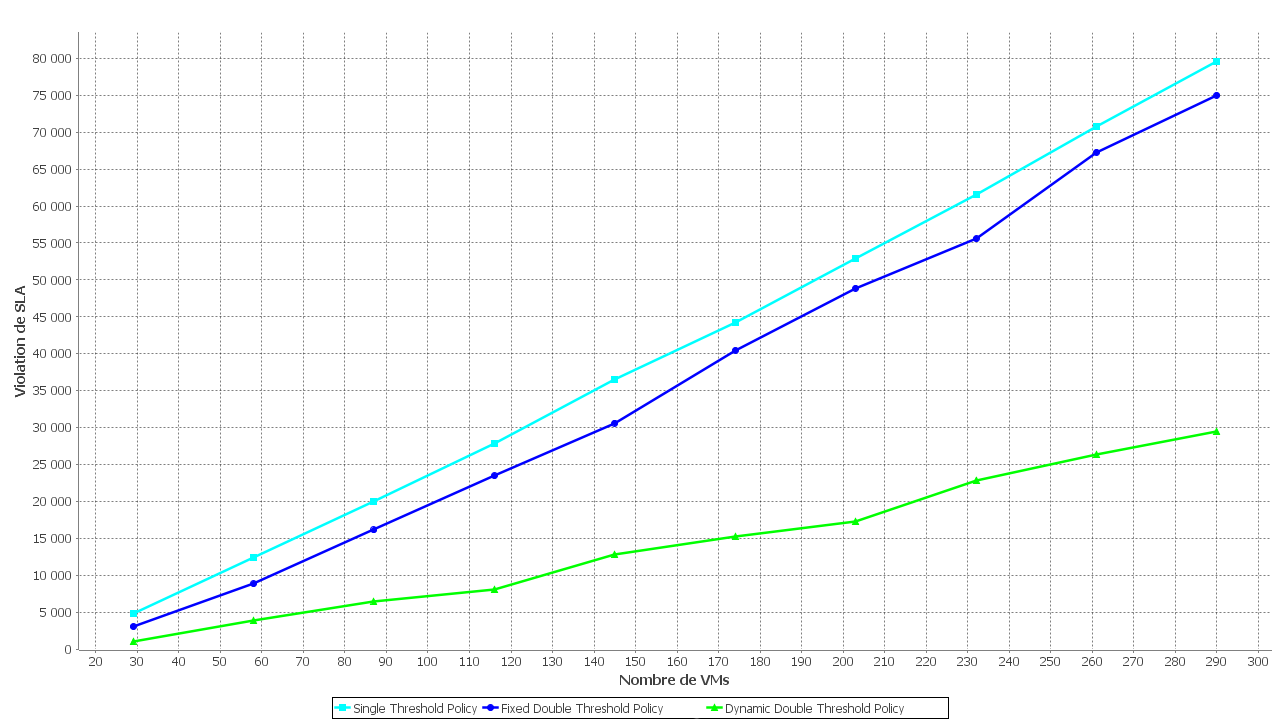
\includegraphics[scale=0.35]{figures/sh3.png} 
\end{center}
\caption{Influence du nombre des VMs sur le nombre de violations de SLA}
\label{InNVMEV}
\end{figure}

Le tableau \ref{GAIN3} montre la différence entre les trois approches, où nous pouvons déduire que notre approche \textbf{Dynamic Double Threshold} a réduit le nombre de violation de SLA avec un gain moyen de 67,35\% par rapport à l'approche \textbf{Single Threshold} et un gain moyen de 61,48\% par rapport à l'approche \textbf{Fixed Double Threshold}.\\


\begin{center}
{\scriptsize   \begin{tabular}{|p{3.5cm}|c|}
\hline
      \centering      Nom de l’approche&  Gain\\
\hline
      \centering      Single Threshold et Dynamic Double Threshold&  67,35\%\\
\hline
      \centering      Fixed Double Threshold et Dynamic Double Threshold&  61,48\%\\
\hline
\end{tabular}}
\captionof{table}{Comparaison entre le nombre de violations de SLA des trois approches}
\label{GAIN3}
\end{center}
Le tableau \ref{PVSLA} montre que l’approche \textbf{Dynamic Double Threshold} a un pourcentage moyen de violation de SLA moins que l’approche \textbf{Single Threshold} et l’approche \textbf{Fixed Double Threshold}.
\begin{center}
{\scriptsize   \begin{tabular}{|p{2.5cm}|c|c|c|c|c|c|c|c|c|c|c|}
\hline
      \centering     Nombre de VMs &  29& 58& 87& 116& 145& 174& 203& 232& 261& 290& Moyen\\
\hline
      \centering      Single Threshold (\%)&  40.83& 41.51& 44.80& 47.39& 48.33& 48.71& 49.33& 49.54& 48.89& 47.81& 46.61\\
\hline
      \centering      Fixed Double Threshold (\%)&  12.92& 17.11& 20.32& 20.48& 22.22& 21.92& 24.41& 25.65& 24.24& 26.82& 21.90\\
\hline
      \centering     Dynamic Double Threshold (\%)&  6.28& 7.37& 7.82& 7.48& 8.57& 8.25& 10.49& 11.40& 10.25& 10.35& 9.12\\
\hline
\end{tabular}}
\captionof{table}{Comparaison entre le pourcentage de violation de SLA des trois approches}
\label{PVSLA}
\end{center}

\subsection{Expérience 2 : Variation du nombre de hôtes}

Pour étudier l’impact du nombre d’hôtes sur la consommation d’énergie, le nombre de migrations et le nombre de violations des SLA, nous avons mesuré les trois principales métriques en appliquant les quatre approches. Nous avons créé un Data Center avec un nombre d’hôtes qui varie de 100 à 280 hôtes avec un pas de 20 où chaque hôte est caractérisée par 1 processeur avec une vitesse variante en MIPS (1000, 2000 ou 3000), 8GB de mémoire, 1TB de stockage et consomme une énergie de 175 W avec 0\% d’utilisation du processeur jusqu’à 250 W avec 100\% d’utilisation du processeur. Le Broker crée pour chaque simulation 290 VMs hétérogènes. Chaque VM possède 1 processeur avec une vitesse variante en MIPS (250, 500, 750 ou 1000), 128MB de mémoire, 1GB de stockage. Nous avons considéré le seuil de l’approche \textbf{Single Threshold} comme 0.6 et les deux seuils supérieur et inférieur de l’approche \textbf{Fixed Double Threshold} comme 0,6 et 0,3 respectivement.


\subsubsection{Consommation d’énergie}
Pour analyser la consommation d’énergie, les résultats obtenus par les simulations sont résumés numériquement dans le tableau \ref{tab5} et schématisés par la Figure \ref{InNVMEn1}. Nous remarquons durant cette série de simulations que les courbes de nos approches se trouvent au-dessous des courbes des autres approches. Donc nos approches sont bien meilleures que  les autres et permettent d’économiser l’énergie consommée.

\begin{center}
{\scriptsize   \begin{tabular}{|p{3.5cm}|c|c|c|c|c|c|c|c|c|c|}
\hline
      \centering     Nombre de PMs &  100& 120& 140& 160& 180& 200& 220& 240& 260& 280\\
\hline
     \centering       Approche sans migration &  35.94& 32.78& 31.34& 30.13& 28.79& 28.68& 28.70& 28.70& 28.67& 28.65\\
\hline
      \centering      Single Threshold &  29.96& 30.10& 28.13& 26.05& 25.37& 24.99& 24.38& 23.84& 23.38& 23.27\\
\hline
      \centering      Fixed Double Threshold &  21.70& 20.57& 19.98& 19.43& 19.13& 19.04& 19.05& 19.06& 19.14& 19.14\\
\hline
      \centering     Dynamic Double Threshold &  17.71& 16.67& 16.60& 16.46& 16.40& 16.39& 16.46& 16.28& 16.42& 16.23\\
\hline
\end{tabular}}
\captionof{table}{Comparaison entre la consommation d’énergie des quatre approches}
\label{tab5}
\end{center}


\begin{figure}[!h]
\begin{center}
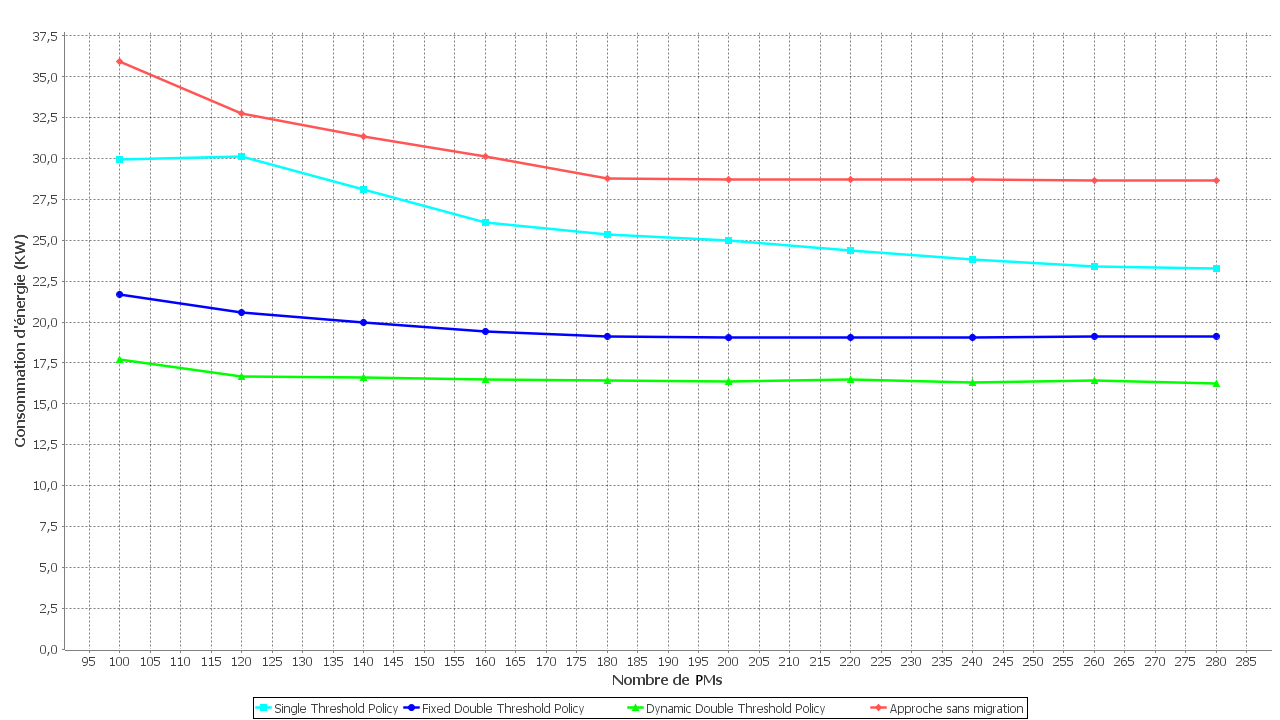
\includegraphics[scale=0.35]{figures/sh4.png} 
\end{center}
\caption{Influence du nombre des PMs sur l’énergie}
\label{InNVMEn1}
\end{figure}

Le tableau \ref{GAIN4} montre la différence entre les quatre approches, où nous pouvons déduire que notre approche \textbf{Dynamic Double Threshold} a réduit l’énergie avec un gain moyen de 45,01\% par rapport à l'approche sans migration, un gain moyen de 35,67\% par rapport à l'approche \textbf{Single Threshold} et un gain moyen de 15,53\% par rapport à l'approche \textbf{Fixed Double Threshold}.\\


\begin{center}
{\scriptsize   \begin{tabular}{|p{3.5cm}|c|}
\hline
      \centering      Nom de l’approche&  Gain\\
\hline
     \centering       Approche sans migration et Dynamic Double Threshold &  45,01\%\\
\hline
      \centering      Single Threshold et Dynamic Double Threshold&  35,67\%\\
\hline
      \centering      Fixed Double Threshold et Dynamic Double Threshold&  15,53\%\\
\hline
\end{tabular}}
\captionof{table}{Comparaison entre la consommation d’énergie des quatre approches}
\label{GAIN4}
\end{center}

\subsubsection{Nombre de migration}
D’après la Figure \ref{InNVMEnM1} et le tableau \ref{tab6}, nous pouvons remarquer que nos approches \textbf{Fixed Double Threshold} et \textbf{Dynamic Double Threshold} ont réduit le nombre de migration par rapport à l’approche \textbf{Single Threshold}.
\begin{center}
{\scriptsize   \begin{tabular}{|p{2.5cm}|c|c|c|c|c|c|c|c|c|c|}
\hline
      \centering     Nombre de PMs & 100& 120& 140& 160& 180& 200& 220& 240& 260& 280\\
\hline
      \centering      Single Threshold &  57883& 61306& 62329& 62475& 62417& 62363& 62432& 62171& 62161& 61992\\
\hline
      \centering      Fixed Double Threshold &  20117& 20269& 20271& 19929& 18984& 19916& 19811& 20009& 19864& 19403\\
\hline
      \centering     Dynamic Double Threshold &  4105& 4273& 3963& 3867& 3937& 3881& 3602& 4222& 4076& 4071\\
\hline
\end{tabular}}
\captionof{table}{Comparaison entre le nombre de migration des quatre approches}
\label{tab6}
\end{center}
\clearpage
\begin{figure}[!h]
\begin{center}
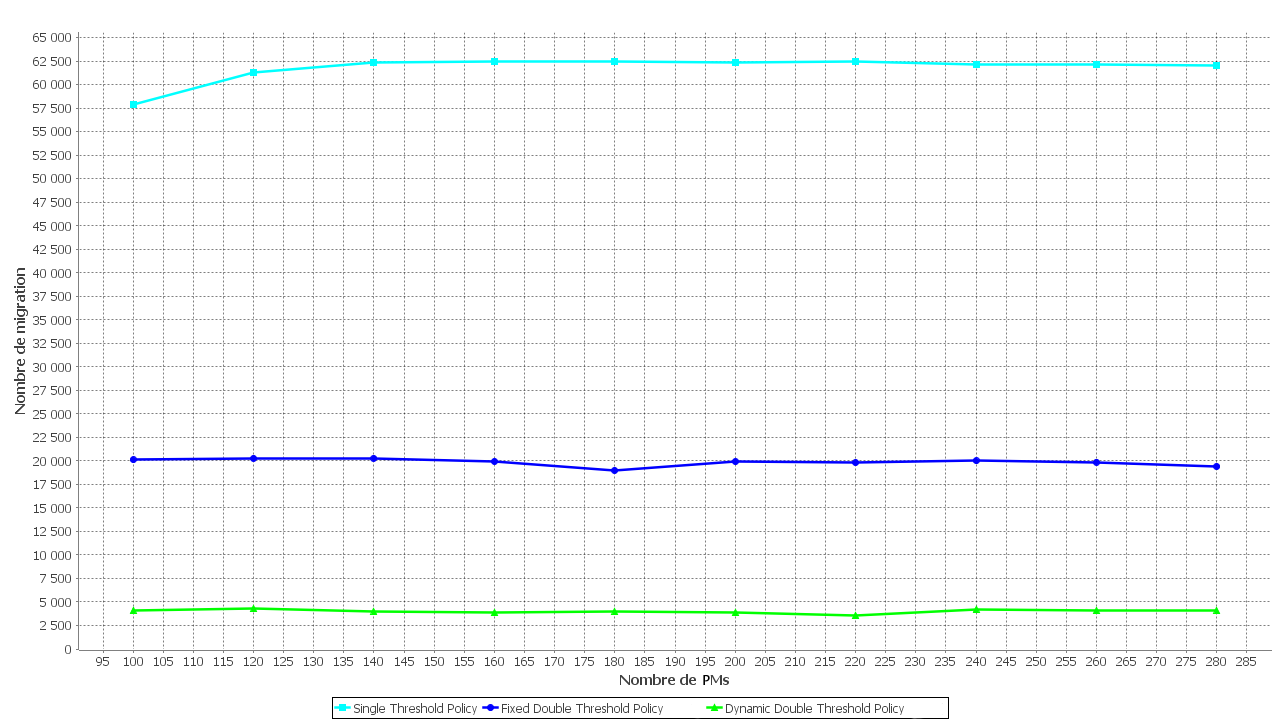
\includegraphics[scale=0.35]{figures/sh5.png} 
\end{center}
\caption{Influence du nombre des PMs sur le nombre de migration}
\label{InNVMEnM1}
\end{figure}


Le tableau \ref{GAIN5} montre la différence entre les trois approches, où nous pouvons déduire que notre approche \textbf{Dynamic Double Threshold} a réduit le nombre de migration avec un gain moyen de 93,51\% par rapport à l'approche \textbf{Single Threshold} et un gain moyen de 79,85\% par rapport à l'approche \textbf{Fixed Double Threshold}.\\

\begin{center}
{\scriptsize   \begin{tabular}{|p{3.5cm}|c|}
\hline
      \centering      Nom de l’approche&  Gain\\
\hline
      \centering      Single Threshold et Dynamic Double Threshold&  93,51\%\\
\hline
      \centering      Fixed Double Threshold et Dynamic Double Threshold&  79,85\%\\
\hline
\end{tabular}}
\captionof{table}{Comparaison entre le nombre de migration des trois approches}
\label{GAIN5}
\end{center}

\subsubsection{Violation de SLA}
La Figure \ref{InNVMEV1} résultante du tableau \ref{tab7} montre que les approches \textbf{Fixed Double Threshold} et \textbf{Dynamic Double Threshold} permettent de minimiser le nombre de violation de SLA par rapport à l’approche \textbf{Single Threshold}.

\begin{center}
{\scriptsize   \begin{tabular}{|p{2.5cm}|c|c|c|c|c|c|c|c|c|c|}
\hline
      \centering     Nombre de PMs &  100& 120& 140& 160& 180& 200& 220& 240& 260& 280\\
\hline
      \centering      Single Threshold &  62422& 63861& 64238& 64087& 64043& 63792& 64065& 63723& 63669& 63346\\
\hline
      \centering      Fixed Double Threshold &  33563& 33200& 32658& 32385& 31741& 32394& 32847& 32401& 32396& 31655\\
\hline
      \centering     Dynamic Double Threshold &  12025& 12637& 11739& 11237& 10863& 11062& 10237& 12238& 11834& 11832\\
\hline
\end{tabular}}
\captionof{table}{Comparaison entre le nombre de violations de SLA des quatre approches}
\label{tab7}
\end{center}

\begin{figure}[!h]
\begin{center}
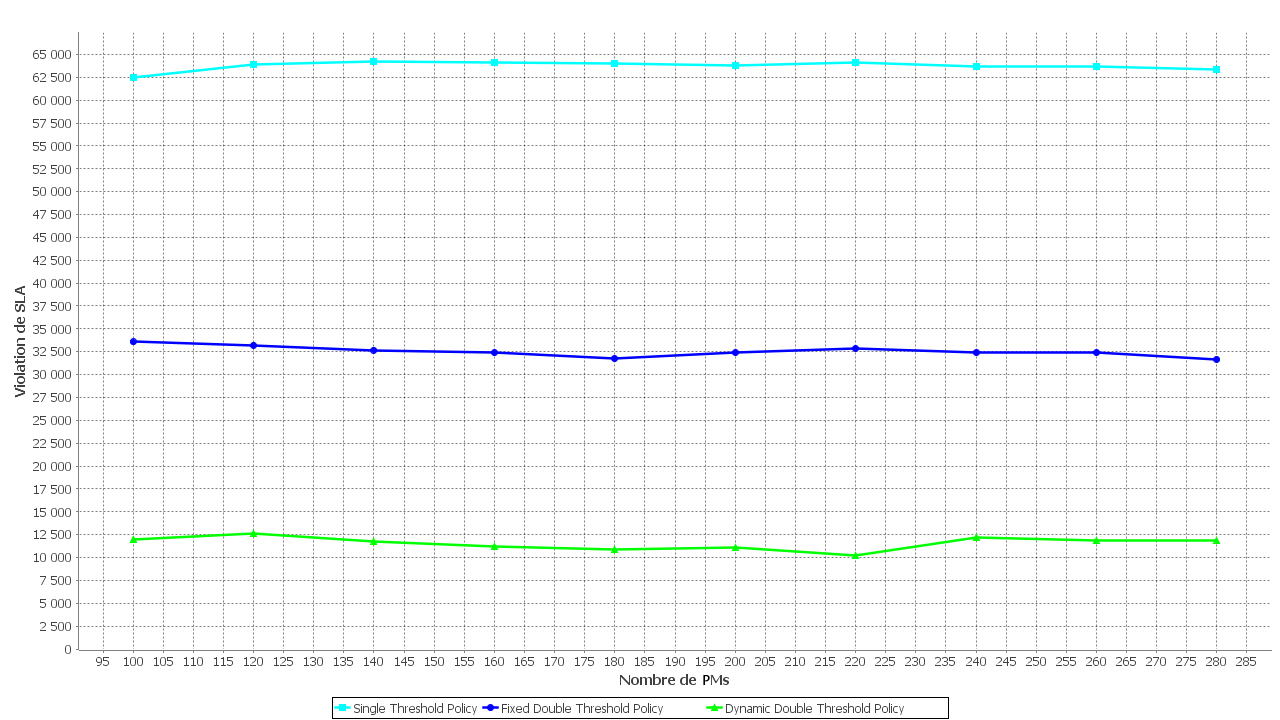
\includegraphics[scale=0.35]{figures/sh6.png} 
\end{center}
\caption{Influence du nombre des PMs sur le nombre de violations de SLA}
\label{InNVMEV1}
\end{figure}

Le tableau \ref{GAIN6} montre la différence entre les trois approches, où nous pouvons déduire que notre approche \textbf{Dynamic Double Threshold} a réduit le nombre de violation de SLA avec un gain moyen de 81,83\% par rapport à l'approche \textbf{Single Threshold} et un gain moyen de 64,42\% par rapport à l'approche \textbf{Fixed Double Threshold}.\\ 
\begin{center}
{\scriptsize   \begin{tabular}{|p{3.5cm}|c|}
\hline
      \centering      Nom de l’approche&  Gain\\
\hline
      \centering      Single Threshold et Dynamic Double Threshold&  81,83\%\\
\hline
      \centering      Fixed Double Threshold et Dynamic Double Threshold&  64,42\%\\
\hline
\end{tabular}}
\captionof{table}{Comparaison entre le nombre de violation de SLA des trois approches}
\label{GAIN6}
\end{center}

Le tableau \ref{PVSLA2} montre que l’approche \textbf{Dynamic Double Threshold} a un pourcentage moyen de violation de SLA moins que l’approche \textbf{Single Threshold} et l’approche \textbf{Fixed Double Threshold}.

\begin{center}
{\scriptsize   \begin{tabular}{|p{2.5cm}|c|c|c|c|c|c|c|c|c|c|c|}
\hline
      \centering     Nombre de PMs &  100& 120& 140& 160& 180& 200& 220& 240& 260& 280& \\
\hline
      \centering      Single Threshold &  47.81& 49.74& 49.87& 50.16& 49.99& 49.87& 49.58& 49.80& 49.55& 49.68& 49.60\\
\hline
      \centering      Fixed Double Threshold &  26.82& 25.29& 25.08& 24.33& 24.92& 25.04& 25.57& 24.87& 25.75& 26.18& 25.21\\
\hline
      \centering     Dynamic Double Threshold &  9.60& 10.00& 9.60& 10.17& 9.70& 9.68& 8.83& 9.90& 9.39& 9.77& 9.66\\
\hline
\end{tabular}}
\captionof{table}{Comparaison entre le pourcentage de violation de SLA des trois approches}
\label{PVSLA2}
\end{center}

\end{onehalfspace}

\section{Conclusion}

\begin{onehalfspace}


Dans ce chapitre, nous avons présenté l’implémentation de notre application ainsi que les résultats obtenus. Aussi, nous avons réalisé plusieurs séries de simulations dans le but de comparer nos approches avec l’approche sans migration et l’approche  \textbf{Single Threshold}   tout en variant différents paramètres comme : le nombre d'hôtes, le nombre de VM. Les résultats de la comparaison ont montré que notre approche permet de minimiser  la consommation d’énergie du système, réduire le nombre de migrations des VMs et par conséquence réduire  le nombre de violations de SLA.

\end{onehalfspace}